\documentclass[tikz]{standalone}

\usepackage{tikz}
\usetikzlibrary{trees}
\usetikzlibrary{shapes}
\usetikzlibrary{positioning}
\usetikzlibrary{arrows.meta}

\tikzset{
    mynode/.style = {circle, ultra thick, draw=black, align=center,fill=yellow!30,font=\ttfamily\bfseries\Large,text=black},
    mynoder/.style = {circle, ultra thick, draw=black, align=center,fill=red!30,font=\ttfamily\bfseries\Large,text=black},
    mynodeb/.style = {circle, ultra thick, draw=black, align=center,fill=blue!30,font=\ttfamily\bfseries\Large,text=black},
    mynodeg/.style = {circle, ultra thick, draw=gray, align=center,fill=gray!05,font=\ttfamily\bfseries\Large,text=gray!20},
    mynodegr/.style = {circle, ultra thick, draw=gray, align=center,fill=gray!05,font=\ttfamily\bfseries\Large,text=red},
    edgen/.style = {-,ultra thick,black},
    edger/.style = {-,ultra thick,red},
    edgeb/.style = {-,ultra thick,blue},
    edgeg/.style = {-,ultra thick,gray},
    edgegd/.style = {-,ultra thick,brown,dashed}, % back
    edgevd/.style = {-,ultra thick,violet,dotted}, % forward
    edgexd/.style = {-,ultra thick,blue,densely dotted}, % traversal
    every picture/.style={/utils/exec={\ttfamily\bfseries}},
    every picture/.style={font issue=\ttfamily\bfseries},
    font issue/.style={execute at begin picture={#1\selectfont}}
}

\newcommand{\R}[1]{\textcolor{red}{#1}}
\newcommand{\B}[1]{\textcolor{violet}{#1}}

\begin{document}

%% 1
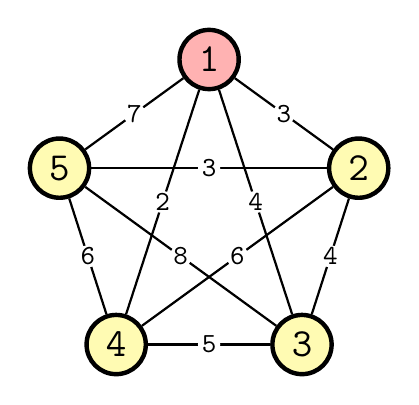
\begin{tikzpicture}[scale=1.00,transform shape]
\node[mynoder] at ( 0.00,  3.00) (1) {1};
\node[mynode] at ( 1.90,  1.62) (2) {2};
\node[mynode] at ( 1.18, -0.62) (3) {3};
\node[mynode] at (-1.18, -0.62) (4) {4};
\node[mynode] at (-1.90,  1.62) (5) {5};

\draw[edgen, thick,-] (1) edge node[fill=white,circle,inner sep=0] {3} (2);
\draw[edgen, thick,-] (1) edge node[fill=white,circle,inner sep=0] {4} (3);
\draw[edgen, thick,-] (1) edge node[fill=white,circle,inner sep=0] {2} (4);
\draw[edgen, thick,-] (1) edge node[fill=white,circle,inner sep=0] {7} (5);
\draw[edgen, thick,-] (2) edge node[fill=white,circle,inner sep=0] {4} (3);
\draw[edgen, thick,-] (2) edge node[fill=white,circle,inner sep=0] {6} (4);
\draw[edgen, thick,-] (2) edge node[fill=white,circle,inner sep=0] {3} (5);
\draw[edgen, thick,-] (3) edge node[fill=white,circle,inner sep=0] {5} (4);
\draw[edgen, thick,-] (3) edge node[fill=white,circle,inner sep=0] {8} (5);
\draw[edgen, thick,-] (4) edge node[fill=white,circle,inner sep=0] {6} (5);

\end{tikzpicture}

%% 2
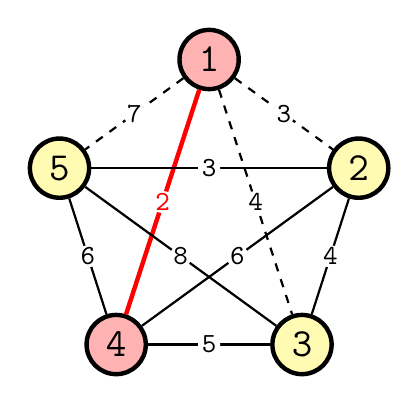
\begin{tikzpicture}[scale=1.00,transform shape]
\node[mynoder] at ( 0.00,  3.00) (1) {1};
\node[mynode] at ( 1.90,  1.62) (2) {2};
\node[mynode] at ( 1.18, -0.62) (3) {3};
\node[mynoder] at (-1.18, -0.62) (4) {4};
\node[mynode] at (-1.90,  1.62) (5) {5};

\draw[edgen, dashed, thick,-] (1) edge node[fill=white,circle,inner sep=0] {3} (2);
\draw[edgen, dashed, thick,-] (1) edge node[fill=white,circle,inner sep=0] {4} (3);
\draw[edger, ultra thick,-] (1) edge node[fill=white,circle,inner sep=0] {2} (4);
\draw[edgen, dashed,thick,-] (1) edge node[fill=white,circle,inner sep=0] {7} (5);
\draw[edgen, thick,-] (2) edge node[fill=white,circle,inner sep=0] {4} (3);
\draw[edgen, thick,-] (2) edge node[fill=white,circle,inner sep=0] {6} (4);
\draw[edgen, thick,-] (2) edge node[fill=white,circle,inner sep=0] {3} (5);
\draw[edgen, thick,-] (3) edge node[fill=white,circle,inner sep=0] {5} (4);
\draw[edgen, thick,-] (3) edge node[fill=white,circle,inner sep=0] {8} (5);
\draw[edgen, thick,-] (4) edge node[fill=white,circle,inner sep=0] {6} (5);

\end{tikzpicture}

%% 3
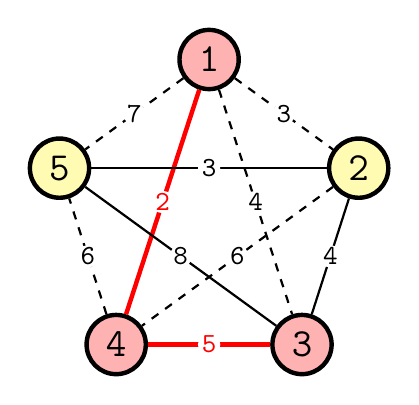
\begin{tikzpicture}[scale=1.00,transform shape]
\node[mynoder] at ( 0.00,  3.00) (1) {1};
\node[mynode] at ( 1.90,  1.62) (2) {2};
\node[mynoder] at ( 1.18, -0.62) (3) {3};
\node[mynoder] at (-1.18, -0.62) (4) {4};
\node[mynode] at (-1.90,  1.62) (5) {5};

\draw[edgen, dashed, thick,-] (1) edge node[fill=white,circle,inner sep=0] {3} (2);
\draw[edgen, dashed, thick,-] (1) edge node[fill=white,circle,inner sep=0] {4} (3);
\draw[edger, ultra thick,-] (1) edge node[fill=white,circle,inner sep=0] {2} (4);
\draw[edgen, dashed,thick,-] (1) edge node[fill=white,circle,inner sep=0] {7} (5);
\draw[edgen, thick,-] (2) edge node[fill=white,circle,inner sep=0] {4} (3);
\draw[edgen, dashed, thick,-] (2) edge node[fill=white,circle,inner sep=0] {6} (4);
\draw[edgen, thick,-] (2) edge node[fill=white,circle,inner sep=0] {3} (5);
\draw[edger, ultra thick,-] (3) edge node[fill=white,circle,inner sep=0] {5} (4);
\draw[edgen, thick,-] (3) edge node[fill=white,circle,inner sep=0] {8} (5);
\draw[edgen, dashed,thick,-] (4) edge node[fill=white,circle,inner sep=0] {6} (5);

\end{tikzpicture}

%% 4
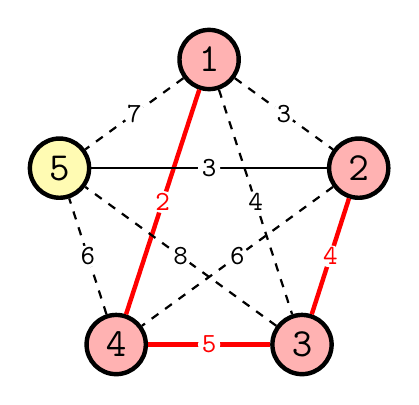
\begin{tikzpicture}[scale=1.00,transform shape]
\node[mynoder] at ( 0.00,  3.00) (1) {1};
\node[mynoder] at ( 1.90,  1.62) (2) {2};
\node[mynoder] at ( 1.18, -0.62) (3) {3};
\node[mynoder] at (-1.18, -0.62) (4) {4};
\node[mynode] at (-1.90,  1.62) (5) {5};

\draw[edgen, dashed, thick,-] (1) edge node[fill=white,circle,inner sep=0] {3} (2);
\draw[edgen, dashed, thick,-] (1) edge node[fill=white,circle,inner sep=0] {4} (3);
\draw[edger, ultra thick,-] (1) edge node[fill=white,circle,inner sep=0] {2} (4);
\draw[edgen, dashed,thick,-] (1) edge node[fill=white,circle,inner sep=0] {7} (5);
\draw[edger, ultra thick,-] (2) edge node[fill=white,circle,inner sep=0] {4} (3);
\draw[edgen, dashed, thick,-] (2) edge node[fill=white,circle,inner sep=0] {6} (4);
\draw[edgen, thick,-] (2) edge node[fill=white,circle,inner sep=0] {3} (5);
\draw[edger, ultra thick,-] (3) edge node[fill=white,circle,inner sep=0] {5} (4);
\draw[edgen, dashed,thick,-] (3) edge node[fill=white,circle,inner sep=0] {8} (5);
\draw[edgen, dashed,thick,-] (4) edge node[fill=white,circle,inner sep=0] {6} (5);

\end{tikzpicture}

%% 5
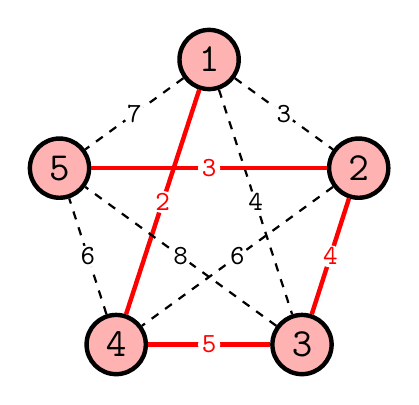
\begin{tikzpicture}[scale=1.00,transform shape]
\node[mynoder] at ( 0.00,  3.00) (1) {1};
\node[mynoder] at ( 1.90,  1.62) (2) {2};
\node[mynoder] at ( 1.18, -0.62) (3) {3};
\node[mynoder] at (-1.18, -0.62) (4) {4};
\node[mynoder] at (-1.90,  1.62) (5) {5};

\draw[edgen, dashed, thick,-] (1) edge node[fill=white,circle,inner sep=0] {3} (2);
\draw[edgen, dashed, thick,-] (1) edge node[fill=white,circle,inner sep=0] {4} (3);
\draw[edger, ultra thick,-] (1) edge node[fill=white,circle,inner sep=0] {2} (4);
\draw[edgen, dashed,thick,-] (1) edge node[fill=white,circle,inner sep=0] {7} (5);
\draw[edger, ultra thick,-] (2) edge node[fill=white,circle,inner sep=0] {4} (3);
\draw[edgen, dashed, thick,-] (2) edge node[fill=white,circle,inner sep=0] {6} (4);
\draw[edger, ultra thick,-] (2) edge node[fill=white,circle,inner sep=0] {3} (5);
\draw[edger, ultra thick,-] (3) edge node[fill=white,circle,inner sep=0] {5} (4);
\draw[edgen, dashed,thick,-] (3) edge node[fill=white,circle,inner sep=0] {8} (5);
\draw[edgen, dashed,thick,-] (4) edge node[fill=white,circle,inner sep=0] {6} (5);

\end{tikzpicture}

%% 6
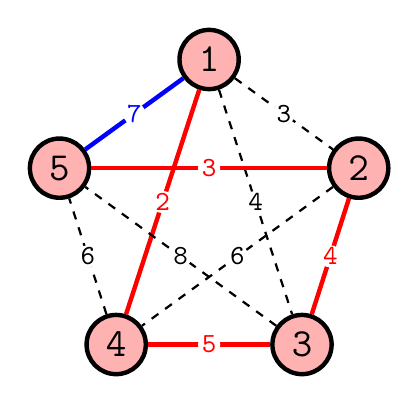
\begin{tikzpicture}[scale=1.00,transform shape]
\node[mynoder] at ( 0.00,  3.00) (1) {1};
\node[mynoder] at ( 1.90,  1.62) (2) {2};
\node[mynoder] at ( 1.18, -0.62) (3) {3};
\node[mynoder] at (-1.18, -0.62) (4) {4};
\node[mynoder] at (-1.90,  1.62) (5) {5};

\draw[edgen, dashed, thick,-] (1) edge node[fill=white,circle,inner sep=0] {3} (2);
\draw[edgen, dashed, thick,-] (1) edge node[fill=white,circle,inner sep=0] {4} (3);
\draw[edger, ultra thick,-] (1) edge node[fill=white,circle,inner sep=0] {2} (4);
\draw[edgeb, ultra thick,-] (1) edge node[fill=white,circle,inner sep=0] {7} (5);
\draw[edger, ultra thick,-] (2) edge node[fill=white,circle,inner sep=0] {4} (3);
\draw[edgen, dashed, thick,-] (2) edge node[fill=white,circle,inner sep=0] {6} (4);
\draw[edger, ultra thick,-] (2) edge node[fill=white,circle,inner sep=0] {3} (5);
\draw[edger, ultra thick,-] (3) edge node[fill=white,circle,inner sep=0] {5} (4);
\draw[edgen, dashed,thick,-] (3) edge node[fill=white,circle,inner sep=0] {8} (5);
\draw[edgen, dashed,thick,-] (4) edge node[fill=white,circle,inner sep=0] {6} (5);

\end{tikzpicture}


\end{document}